
\FloatBarrier

\section{Система Чуа} %% {{{1 _CHUA_
\label{atu:sect:chua}

\LinkRef{
 chua: ASAU-18, MKMM-2014, APIR-2011
}

\subsection{Визначення системи та аналіз її динаміки} % {{{2 _chua_task

Однією з відомих хаотичних систем, легко реалізованих як аналітично,
(\ref{atu:eq:chua}), так і схемотехнічно (рис.~\ref{atu:f:chuascheme}),
є нелінійна система Чуа~\cite{moon_chaotic_vibr,buga_chua,Kennedy92robustop,Kennedy_Chua_primer}:

\begin{figure}[htb!]
\begin{center}
% vi:syntax=tex

\begin{circuitikz}[line width=0.7]
  \ctikzset{bipoles/thickness=2}
  \def\Top{3.0}
  \draw (0.0,0.0) to[L,l=$L$,i=$I_L$] (0,\Top)
   to[R=R] (6.0,\Top)
   to[ageneric,l=$R_c$] (6.0,0.0) -- (0.0,0.0);
  \draw(1.5,0.0) to[C,l=$C_2$,v=$V_2$] (1.5,\Top );
  \draw(4.5,0.0) to[C,l=$C_1$,v=$V_1$] (4.5,\Top );
\end{circuitikz}

% \begin{tikzpicture}[circuit ee IEC,very thick,circuit symbol unit=3.5mm]
%   \node (L1) at (0,1.5) [point up,elelem,inductor={info = $L$}] {};
%   \node      at (0.2,2.4) {$I_L$};
%   \node (C2) at (1.5,1.5) [point up,elelem,capacitor={info = $C_2$}] {};
%   \node      at (1.8,1.8) {$V_2$};
%   \node (pc2d) at (1.5,0) [contact] {};
%   \node (pc2u) at (1.5,3) [contact] {};
%   \node (C1) at (5.0,1.5) [point up,elelem,capacitor={info = $C_1$}] {};
%   \node      at (5.3,1.8) {$V_1$};
%   \node (pc1d) at (5,0) [contact] {};
%   \node (pc1u) at (5,3) [contact] {};
%   \node (R) at (3,3) [elelem,resistor={info = $R$}] {};
%   \node (Rc) at (7,1.5) [elelem,point up,resistor={info = $R_c$}] {};
%   \draw (Rc) ++(-0.15,-0.7) rectangle+(0.3,0.2);
%   \draw (L1) |- (pc2d) -- (pc1d) -| (Rc) [wire];
%   \draw (L1) |- (pc2u) -- (R) -- (pc1u) -| (Rc) [wire];
%   \draw (pc2u) -- (C2) [wire]; \draw (pc2d) -- (C2) [wire];
%   \draw (pc1u) -- (C1) [wire]; \draw (pc1d) -- (C1) [wire];
%   \node (Gr) at (5,-0.3) [elelem,point down,ground] {};
%   \draw (pc1d) -- (Gr) [wire];
% \end{tikzpicture}

\end{center}
\caption{Умовна електричний ланцюг, що реалізує хаотичну систему Чуа}
\label{atu:f:chuascheme}
\end{figure}


\begin{equation}
\begin{cases}
  C_1 \dot{V_1}  = \frac{1}{R} ( V_2 - V_1 ) - g(V_1), \\
  C_2 \dot{V_2}  = \frac{1}{R} ( V_1 - V_2 ) + I_L, \\
  \dot{I_L}      = - \frac{1}{L} V_2 .
\end{cases}
\label{atu:eq:chua}
\end{equation}

Єдиним нелінійним елементом в цій системі є ``діод Чуа''
(позначений на схемі як $R_c$) з
характеристикою
$g(V)$~(рис.~\ref{atu:f:diodchua}),
характеризується різними від'ємними нахилами ($m_0 $ і $ m_1 $)
на різних ділянках, і тим самим виступає у ролі керованого джерела енергії.
%
\begin{equation}
g(V) =
\begin{cases}
  m_1 V = ( m_0 + m_2 ) V , & |V| <   U_0, \\
  m_0 V ,                   & |V| \ge U_0.
\end{cases}
\label{atu:eq:diodchua}
\end{equation}

\begin{figure}[htb!]
\begin{center}
% vi:syntax=tex
\begin{tikzpicture}
  \coordinate (XMIN) at (-4.5,0.0);
  \coordinate (XMAX) at ( 4.5,0.0);
  \coordinate (YMIN) at (0,-2.5);
  \coordinate (YMAX) at (0, 2.5);
  \draw (XMIN) -- (XMAX) [medline,->] node[below] {$U$};
  \draw (YMIN) -- (YMAX) [medline,->] node[left]  {$I$};
  \draw (-4,2) -- (-1,1) -- (1,-1) -- (4,-2) [boldline];
  \draw (1,-1) -- (1,0) [dashed,medline];
  \draw (1,-1) -- (4,-1) [dashed,medline];
  \draw (1.41,0) arc [medline,->,start angle=0,end angle=-45,radius=1.41];
  \draw (1,-1) ++(2,0) arc [medline,->,start angle=0,end angle=-18,radius=2.0];
  \filldraw (1,0) circle[radius=0.05,fill=black] node[above] {$U_0$};
  \node[right] at (1.2,-0.6) {$\alpha_1: \tan(\alpha_1)=m_1$};
  \node[right] at (3.0,-1.3) {$\alpha_0$};
\end{tikzpicture}

\end{center}
\caption{Характеристика \(I = g (V) \) діода Чуа}
\label{atu:f:diodchua}
\end{figure}


При цьому параметр \(m_0\) визначає надходження енергії в
систему при великих амплітудах \(V_1\), і, в цілому, характеризує
енергетичні можливості джерела. Аналогічно, параметр \(m_1\)
характеризує надходження енергії при малих коливаннях, зокрема,
визначає, чи буде система переходити в коливальний стан при
малих початкових збурень, і якою буде режим цих коливань. З
іншого боку, оскільки параметр \(m_1\) є сумою ``глобального
параметра'' \(m_0 \) і ``доважку'', що визначає додатковий внесок
при малих амплітудах, то має сенс перейти від параметра \(m_1 \) до
параметру \(m_2 = m_1 - m_0 \), який і визначає в цілому нелінійність
системи. При \(m_2 = 0 \) система стає лінійною і не представляє
особливого інтересу.
У даній роботі як параметр, що підлягає ідентифікації, обрано саме~$m_2$.

Відомо, що в залежності від величини параметра
$ m_2 $, система може переходити в режими загасання, періодичного
і складно-періодичного руху, а також в режим хаотичних
коливань~\cite{anisch_nonlin_eff,magni_new_meth,Chua_double_scroll}. При цьому
складно-періодичний і хаотичний рух чергуються зі зміною
величини \(m_2\).


Класично параметри системи Чуа задаються наступним чином~\cite{buga_chua}:
$C_1 = 1/9$, $C_2 = 1$, $L= 1/7$, $R = 1/0.7$, $m_0=-0.5$, $ m_2 \in [ -0.15; -0.7 ] $.

Введемо позначення:
\[
  a_{11} = \frac{1}{R C_1}; \;
  a_{13} = \frac{1}{C_1}; \;
  a_{21} = \frac{1}{R C_2}; \;
  a_{23} = \frac{1}{C_2}; \;
  a_{31} = -\frac{1}{L}; \;
  a_g = - \frac{m_0}{C_1}; \;
  \mu = - \frac{m_2}{C_1}.
\]
%
%\noindent
Тоді:
%
\begin{equation}
\begin{cases}
  \dot{V}_1  = -a_{11} V_1 + a_{11}  V_2  + g_1(V_1) , \\
  \dot{V}_2  = +a_{21} V_1 - a_{21}  V_2  + a_{23} I_L    , \\
  \dot{I}_L  =  a_{31} V_2.
\end{cases}
\label{atu:eq:chua2}
\end{equation}
%
%
\begin{equation}
g_1(V) =
\begin{cases}
  ( a_g + \mu ) V , & |V| <   U_0, \\
  a_g V           , & |V| \ge U_0.
\end{cases}
\label{atu:eq:diodchua2}
\end{equation}

При цьому перелічені класичні значення параметрів будуть представлені таким чином:
$ a_{11} = 6.5 $, $a_{21} = 0.7$, $ a_{23} = -7 $, $ a_g = 4.5 $,
$ \mu \in [ 1.29 ; 5.6 ] $.
Відповідно, в цих позначеннях ідентифікований параметр є~$\mu$. Він задає вид динаміки системи.


\begin{figure}[htb!]
\centerline{
  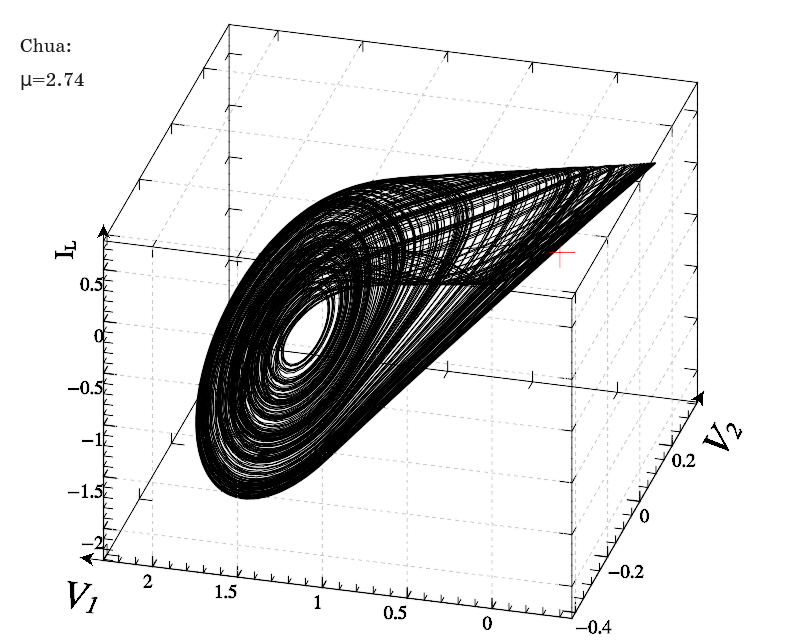
\includegraphics[width=0.49\textwidth]{p/cha/chua/chua_1-p_xyz_mu=2x74.png}
  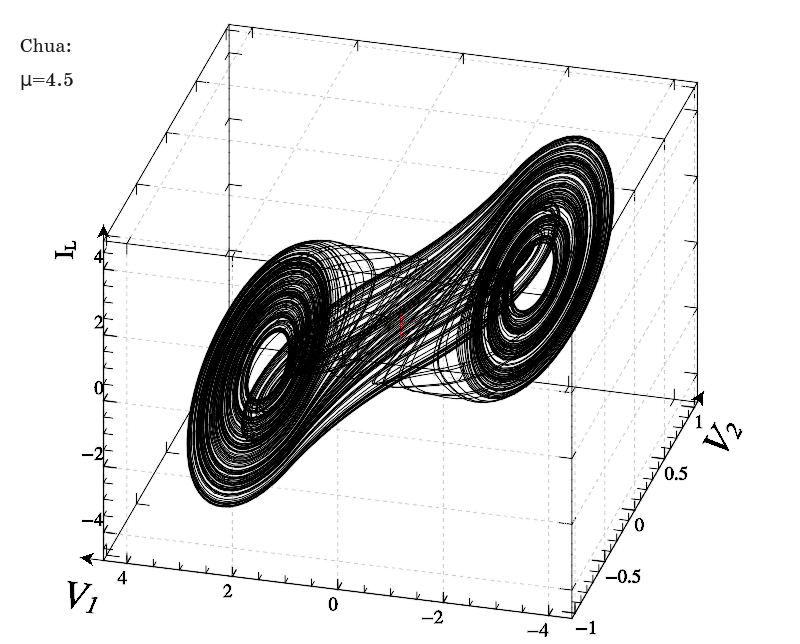
\includegraphics[width=0.49\textwidth]{p/cha/chua/chua_1-p_xyz_mu=4x50.png}
}
\caption{Аттрактор системи Чуа (\ref{atu:eq:chua2}) при різних значеннях $ \mu $}
\label{atu:f:chua_phase}
\end{figure}


% }}}2

\subsection{Аналіз і вибір критеріїв}%{{{2


Для визначення виду критерію розглянемо залежності
$q_{*}(\mu)$ (індексом ``*'' будемо позначати застосування будь-якого
з індексів, що позначають вихідний сигнал для критерію і спосіб
усереднення), отримані шляхом моделювання для системи Чуа (рис.~\ref{atu:f:chua_q}):

\begin{figure}[htb!]
\centerline{
  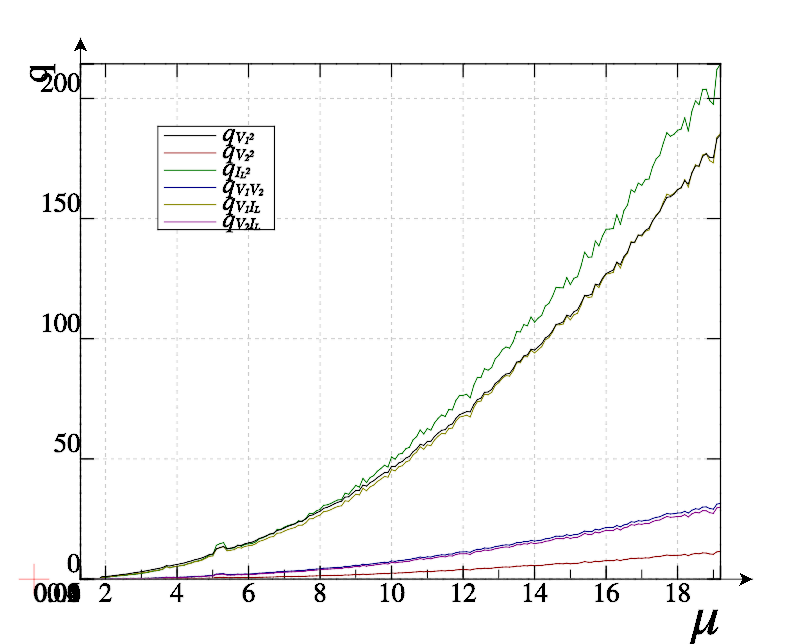
\includegraphics[width=0.49\textwidth]{p/cha/chua/chua_q-p_mu2.png}
  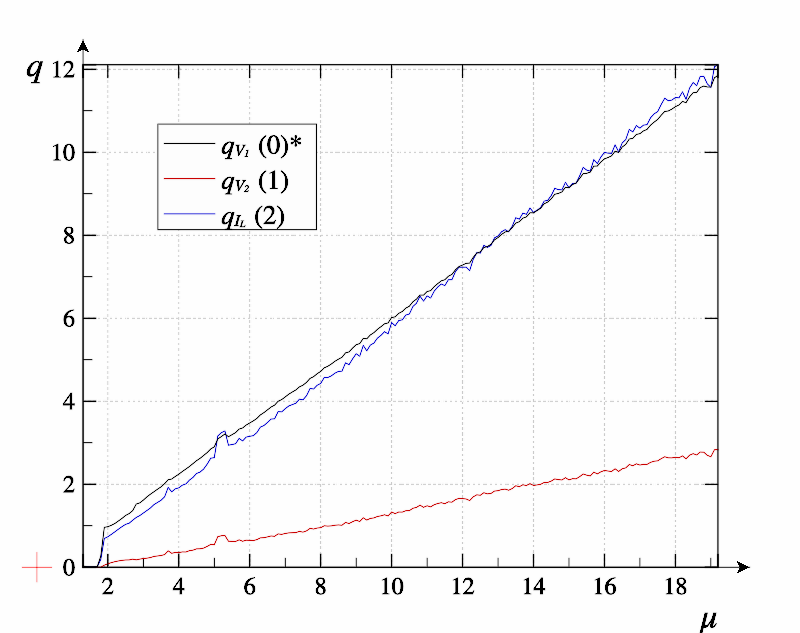
\includegraphics[width=0.49\textwidth]{p/cha/chua/chua_q-p_mu1.png}
}
\caption{Залежності $ q_{*} (\mu) $ для системи Чуа (\ref{atu:eq:chua2})}
\label{atu:f:chua_q}
\end{figure}

З аналізу графіків зроблено висновок, що величина $q_{V_1}(\mu)$
є найкращим кандидатом в критерії, з огляду на близьку до
лінійної залежності в робочому діапазоні~\cite{atu_apir2011}.

Наступним важливим параметром, необхідним для ефективної
роботи системи ідентифікації, є характерний час оцінювання
$ \tau $ (\ref{atu:eq:qlin}), або ж зворотна йому величина
$ a_q $.

Для попереднього оцінювання величини
$ a_q $ розглянемо спектри системи при різних
$ \mu $ (рис.~\ref{atu:f:chua_spectrum}). Як випливає з графіків, спектр системи
досить обмежений зверху, проте, в хаотичному режимі є суцільним
практично до нуля. Це не дає можливості безпосередньо визначити
$ a_q $ виходячи із спектру, однак, перші суттєві піки
спостерігаються при
$ \omega \approx 0.3 $, отже, первинне значення
$ a_q $ можна оцінити як
$ a_q \approx 0.3 / \pi \approx 0.1 $ .


\begin{figure}[htb!]
\centerline{
  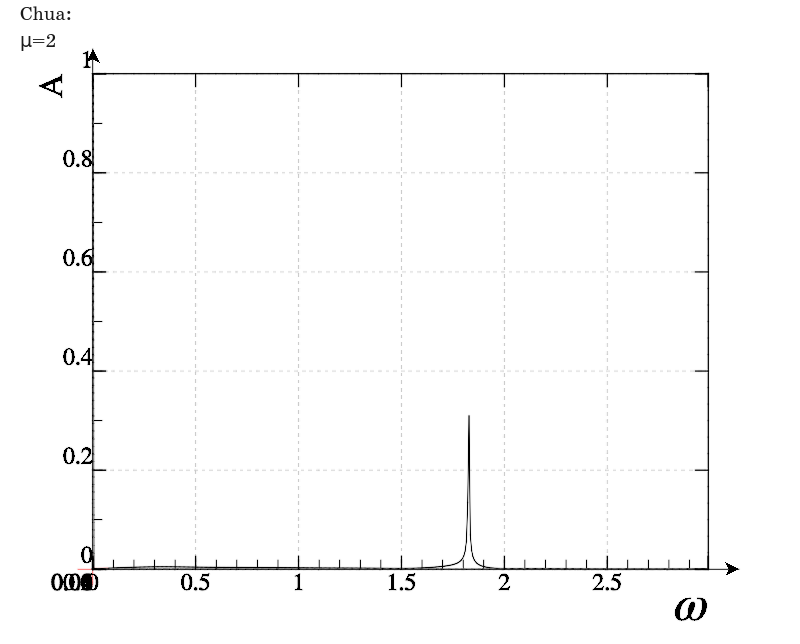
\includegraphics[width=0.32\textwidth]{p/cha/chua/chua_f-p_f_mu=2x00.png}
  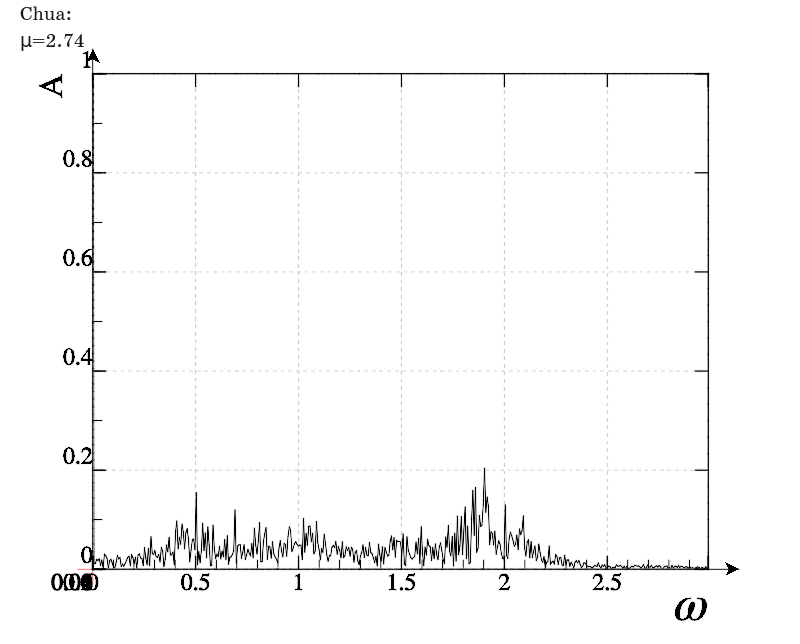
\includegraphics[width=0.32\textwidth]{p/cha/chua/chua_f-p_f_mu=2x74.png}
  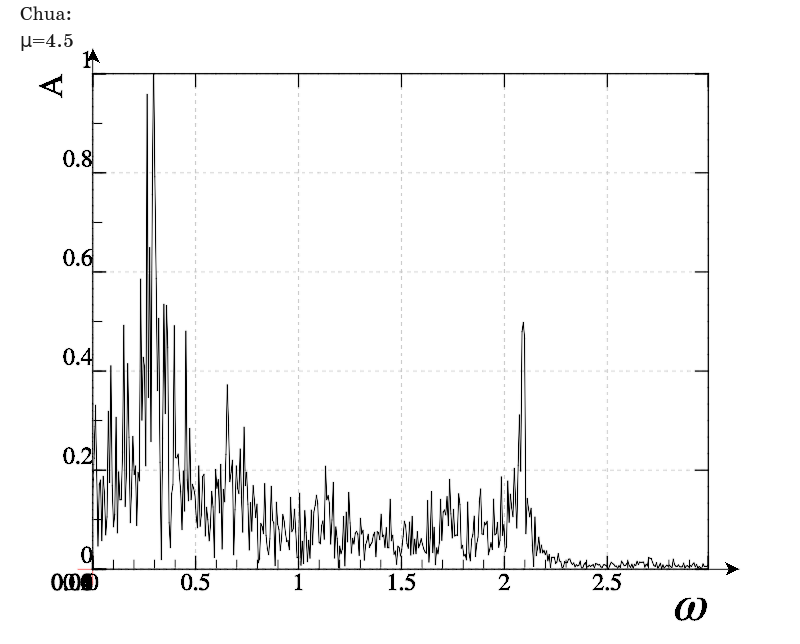
\includegraphics[width=0.32\textwidth]{p/cha/chua/chua_f-p_f_mu=4x50.png}
}
\caption{Спектри системи Чуа (\ref{atu:eq:chua2}) при різних значеннях $ \mu $}
\label{atu:f:chua_spectrum}
\end{figure}

Наступний спосіб оцінити
$ a_q $ --- дослідити отриману в результаті моделювання залежність
середньоквадратичного відхилення
$ e_q $ оцінки величини
$ q $, нормованої на саму величину
$ q $ в стаціонарному випадку. Отримана залежність представлена
на рис.~\ref{atu:f:chua_tau}.

\begin{figure}[htb!]
\centerline{
  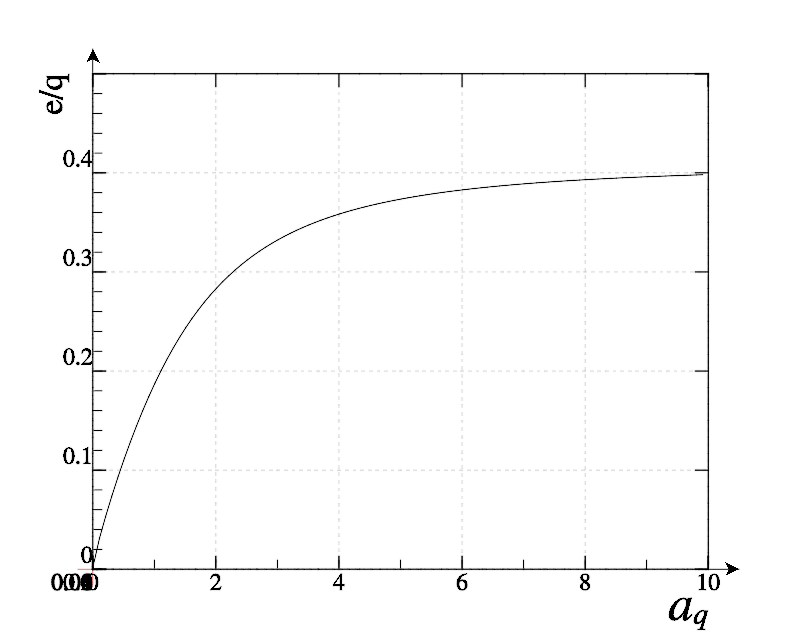
\includegraphics[width=0.4\textwidth]{p/cha/chua/chua_tau-p_e_a.png}
}
\caption{Типова залежність $ e_q / q (a_q) $ для системи (\ref{atu:eq:chua2})}
\label{atu:f:chua_tau}
\end{figure}

З цього графіка можна зробити висновок, що первісна оцінка $ a_q $ була зроблена коректно.

% }}}2

\subsection{Тестова задача ідентифікації для системи Чуа}%{{{2

Відповідно до отриманих даних, і використовуючи
пропозиції~(\ref{atu:eq:po_t_sign}) і~(\ref{atu:eq:po_t_sin}), визначимо тестове
завдання наступним чином:
%
\begin{equation}
 \mu_o(t) = p_0 + U_p \sign \sin( \omega_p t )
  \label{atu:eq:chua_mu_sign}
\end{equation}
%
\begin{equation}
 \mu_o(t) = p_0 + U_p \sin( \omega_p t ).
  \label{atu:eq:chua_mu_sin}
\end{equation}
%
де:
$p_0 = 3.25$, $U_p=0.6$, $\omega_p = \pi / 300$.

При моделюванні процесів ідентифікації було виявлено наступне
явище: якщо динаміка параметра
$ \mu $ задана (\ref{atu:eq:chua_mu_sign}), то існують такі значення
$ p_0 $ і $ U_p $, при яких система повністю втрачає стійкість. Для
схемотехнічних реалізацій системи Чуа таких явищ не
спостерігається, так як реальні системи мають обмежені
можливості з підтримки від'ємного опору. Для таких
випадків подання діода Чуа у вигляді (\ref{atu:eq:diodchua}) не є
адекватним~\cite{atu_kher2014}. Точніше, з огляду на той факт, що
схемотехнічні реалізації з'явилися після аналітичного
дослідження, більш правильним буде твердження про те, що реалізації
недостатньо адекватно реалізують аналітичну залежність
для діода Чуа. Більш адекватна реалізація вимагає наявності
необмеженого джерела енергії. З урахуванням вищезазначеного,
множина тестових систем для даної задачі є більш обмеженою.

На рис.~\ref{atu:f:chua_id_ql3rlWvnAAW_sign} представлені результати
моделювання процесу ідентифікації групою методів ql3rlWvnAAW за
умови~(\ref{atu:eq:chua_mu_sign}).

\begin{figure}[htb!]
  \centerline{
    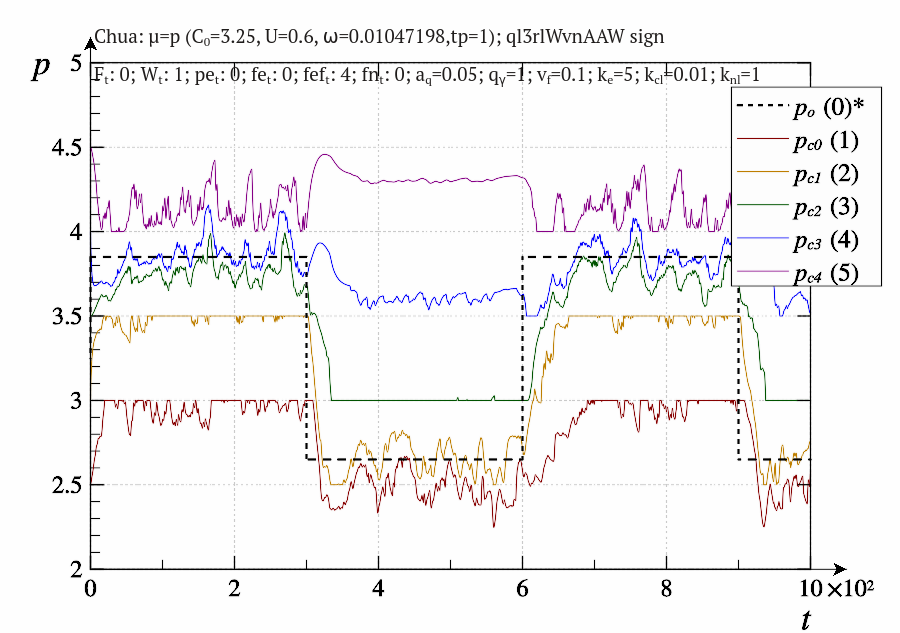
\includegraphics[width=0.49\textwidth]{p/cha/chua/ql3rlWvnAAW/chua_id-p_t_pi_ql3rlWvnAAW_sign.png}
    \hfill
    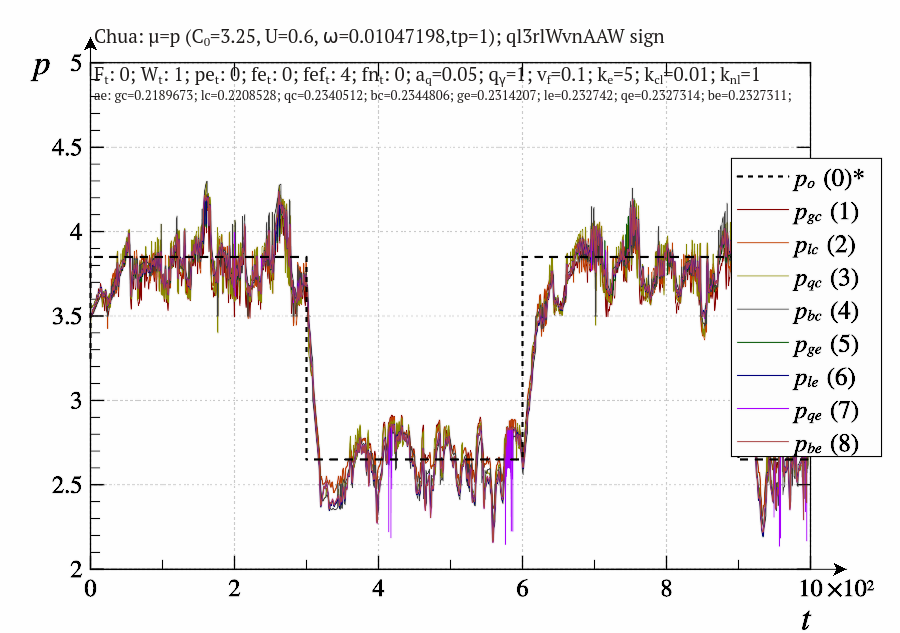
\includegraphics[width=0.49\textwidth]{p/cha/chua/ql3rlWvnAAW/chua_id-p_t_p_ql3rlWvnAAW_sign.png}
  }
\caption{Процес ідентифікації параметра ``$\mu$'' системи Чуа групою методів ql3rlWvnAAW за умови~(\ref{atu:eq:chua_mu_sign})}
  \label{atu:f:chua_id_ql3rlWvnAAW_sign}
\end{figure}

При заданих умовах система цілком працездатна, рівень коливань
ідентифікованого параметра цілком відповідає задачі.

На рис.~\ref{atu:f:chua_id_ql3rlWvnAAW_sin} представлені результати
моделювання процесу ідентифікації групою методів ql3rlWvnAAW за
умови~(\ref{atu:eq:chua_mu_sin}).

\begin{figure}[htb!]
  \centerline{
    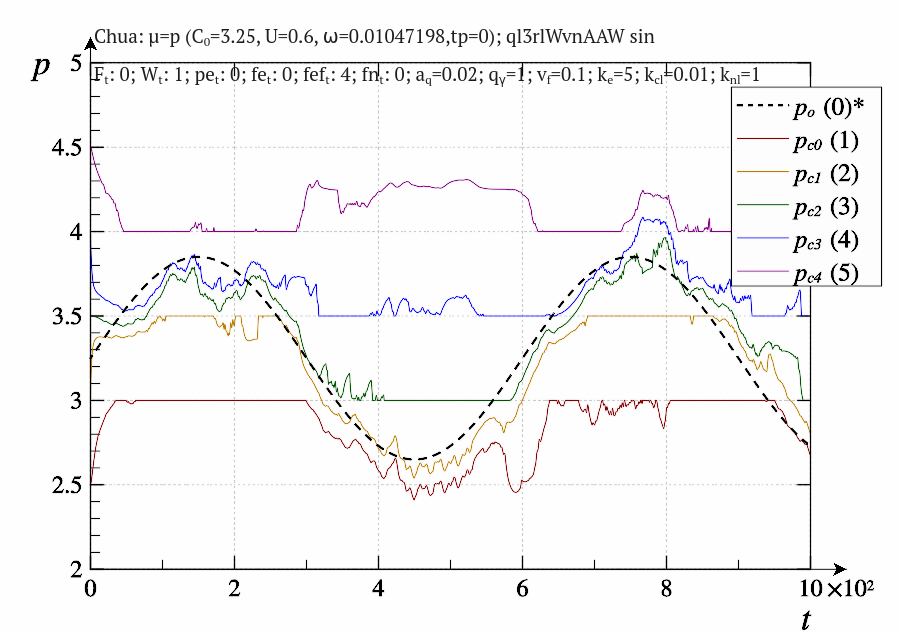
\includegraphics[width=0.49\textwidth]{p/cha/chua/ql3rlWvnAAW/chua_id-p_t_pi_ql3rlWvnAAW_sin.png}
    \hfill
    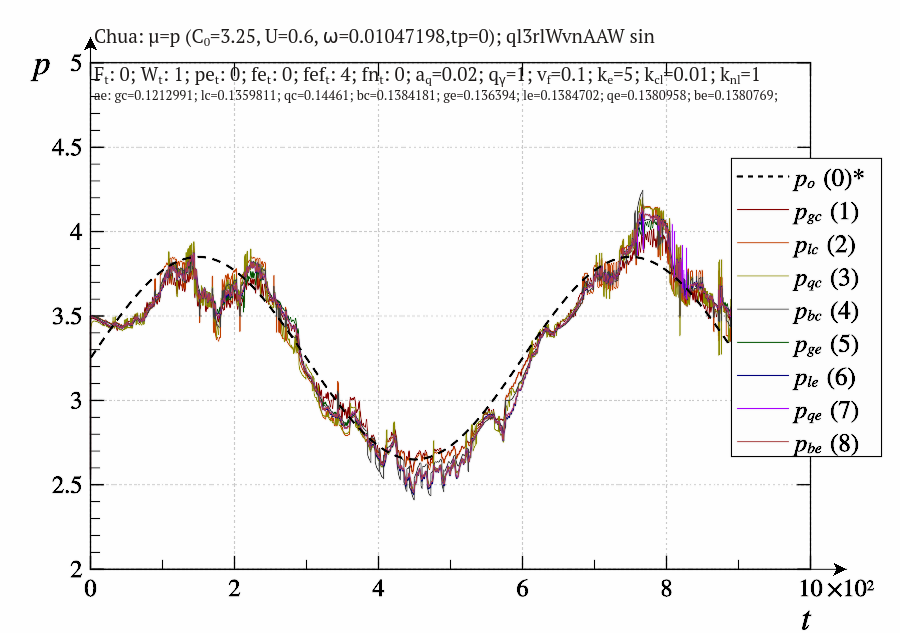
\includegraphics[width=0.49\textwidth]{p/cha/chua/ql3rlWvnAAW/chua_id-p_t_p_ql3rlWvnAAW_sin.png}
  }
\caption{Процес ідентифікації параметра ``$\mu$'' системи Чуа групою методів ql3rlWvnAAW за умови~(\ref{atu:eq:chua_mu_sin})}
\label{atu:f:chua_id_ql3rlWvnAAW_sin}
\end{figure}

Як загальний рівень похибки, так і розмах коливань значення
параметра в цьому випадку помітно менше, аналогічно процесам
ідентифікації інших розглянутих хаотичних систем.

Процес ідентифікації в умовах, коли параметр
$ \mu $ повільно і лінійно ``пробігає'' увесь робочий
діапазон, що підлягає аналізу, проілюстрований на рис.~\ref{atu:f:chua_id_ql3rlWvnAAW_ramp}.

\begin{figure}[htb!]
  \centerline{
    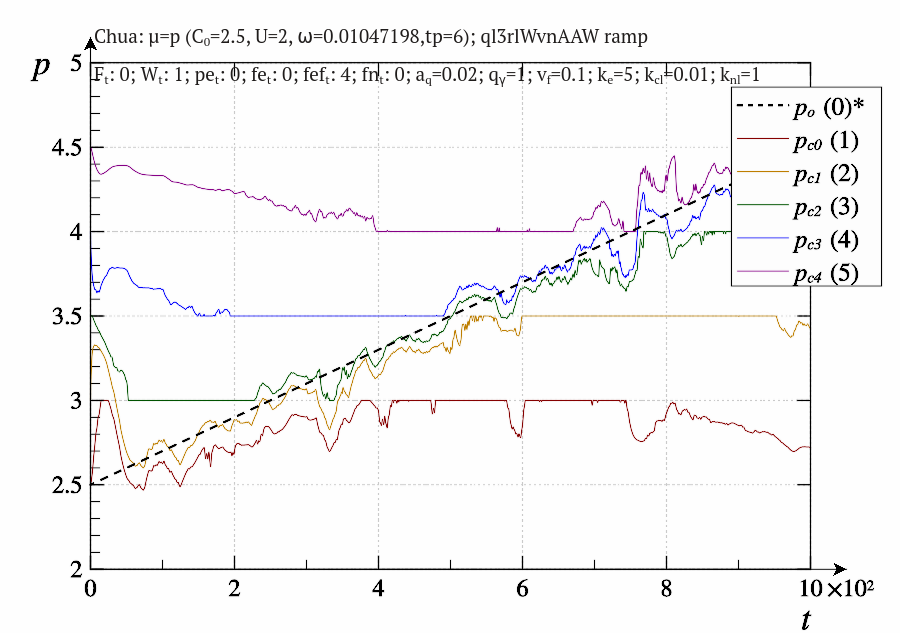
\includegraphics[width=0.49\textwidth]{p/cha/chua/ql3rlWvnAAW/chua_id-p_t_pi_ql3rlWvnAAW_ramp.png}
    \hfill
    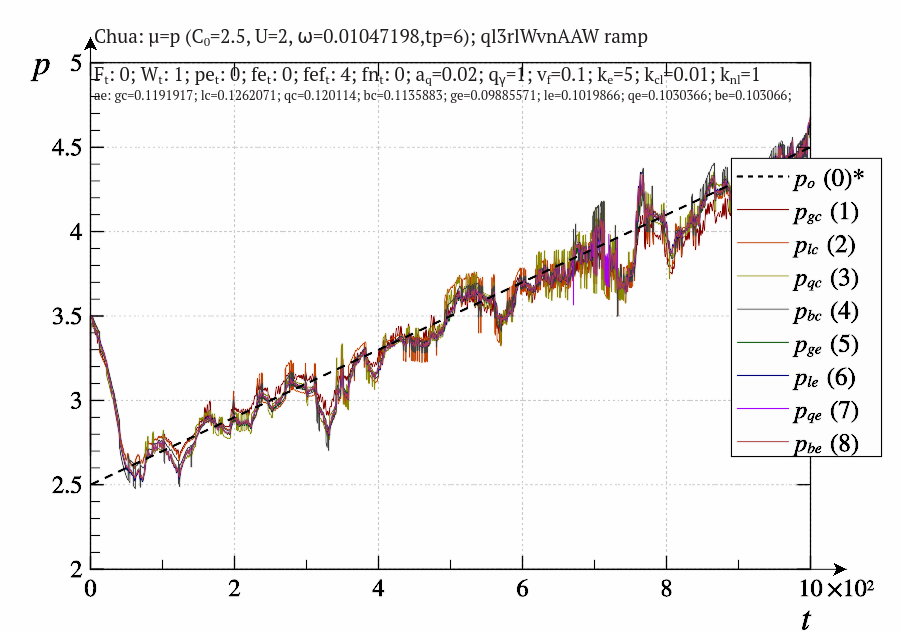
\includegraphics[width=0.49\textwidth]{p/cha/chua/ql3rlWvnAAW/chua_id-p_t_p_ql3rlWvnAAW_ramp.png}
  }
\caption{Процес ідентифікації параметра ``$\mu$'' системи Чуа групою методів ql3rlWvnAAW за умови~(\ref{atu:eq:po_t_ramp})}
\label{atu:f:chua_id_ql3rlWvnAAW_ramp}
\end{figure}

Залежності на графіках свідчать про те, що з урахуванням рівня
похибки, ідентифікація на всьому діапазоні відбувається без
будь-яких істотних порушень.


% }}}2


\subsection{Вплив параметрів системи ідентифікації на похибку ідентифікації для системи Чуа} % {{{2

Для більш точного налаштування параметрів самої системи
ідентифікації розглянемо залежності помилок ідентифікації
від основних параметрів системи ідентифікації.

Для перевірки коректності вибору величини
$ a_q $ були побудовані залежності помилок ідентифікації
(рис.~\ref{atu:f:chua_e_a_q}) від цього параметра.


\begin{figure}[htb!]
  \centerline{
    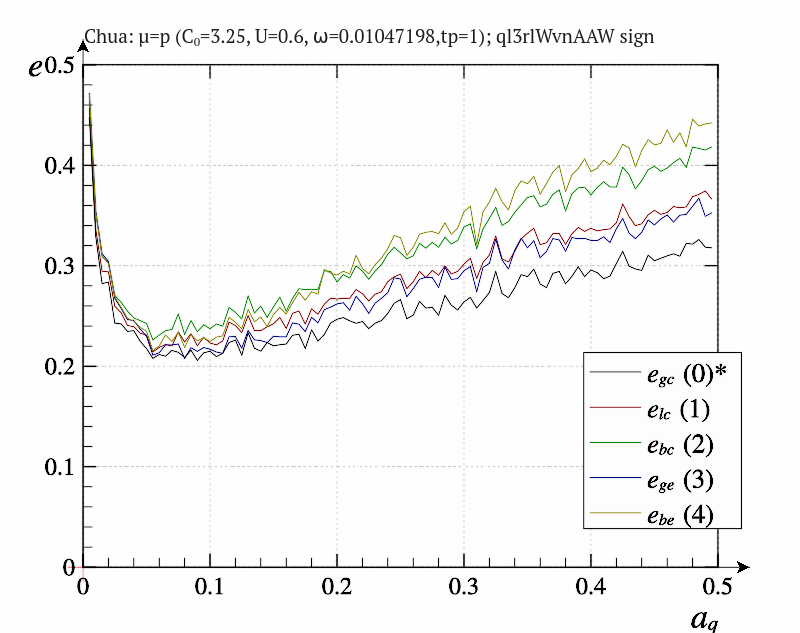
\includegraphics[width=0.49\textwidth]{p/cha/chua/ql3rlWvnAAW/chua_id-p_a_q_sign.png}
    \hfill
    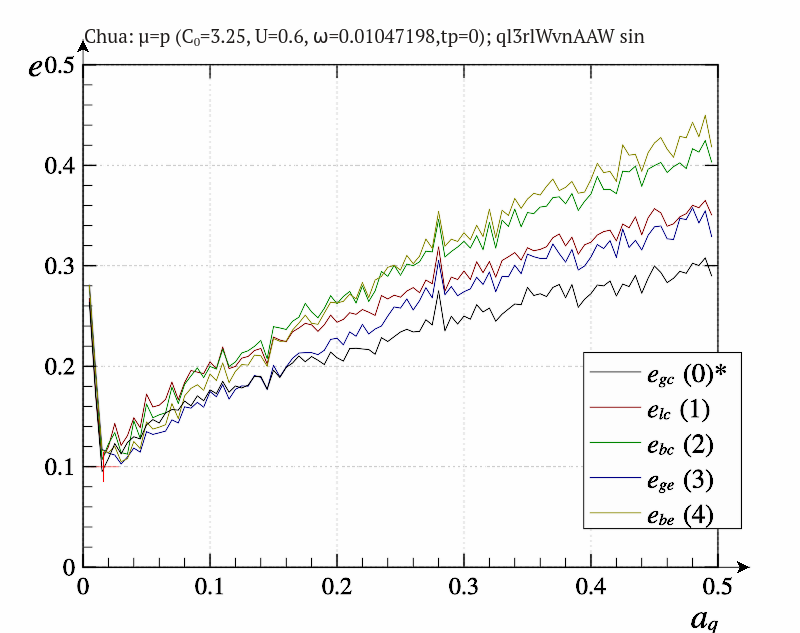
\includegraphics[width=0.49\textwidth]{p/cha/chua/ql3rlWvnAAW/chua_id-p_a_q_sin.png}
  }
\caption{Залежності $ \overline{e} (a_q) $ для системи (\ref{atu:eq:chua2}) при умовах (\ref{atu:eq:chua_mu_sign}) і (\ref{atu:eq:chua_mu_sin})
}
\label{atu:f:chua_e_a_q}
\end{figure}

Як видно з результатів моделювання, первісна оцінка ``коректного'' значення величини
$a_q$ була зроблена досить точно. При цьому, при синусоїдальній
зміні параметра об'єкта менша похибка ідентифікації
спостерігається при менших значеннях
$ a_q $, що пов'язано з тим, в даному випадку немає необхідності в
стеженні за параметром, величина якого стрибкоподібно змінюється,
і, отже, припустим більший час оцінювання. Навпаки, в разі
(\ref{atu:eq:chua_mu_sign}) збільшення часу оцінювання призводить до
помітного зниження інтегральної точності ідентифікації.


Одним з найважливіших параметрів є
$ q_\gamma $ --- масштаб функції якості
((\ref{atu:eq:F_gauss})--(\ref{atu:eq:F_log})).
Залежності для цього параметра наведені на рис.~\ref{atu:f:chua_e_qgamma}.

\begin{figure}[htb!]
  \centerline{
    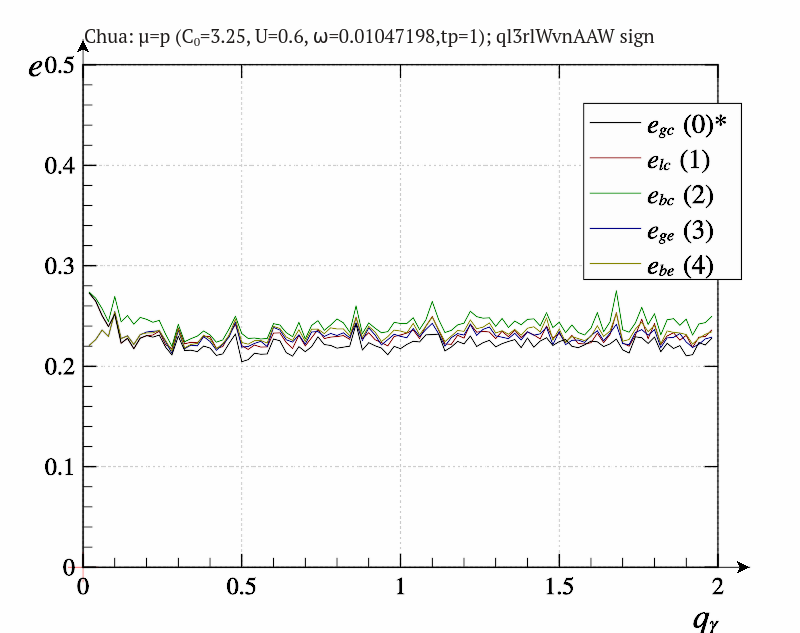
\includegraphics[width=0.49\textwidth]{p/cha/chua/ql3rlWvnAAW/chua_id-p_q_gamma_sign.png}
    \hfill
    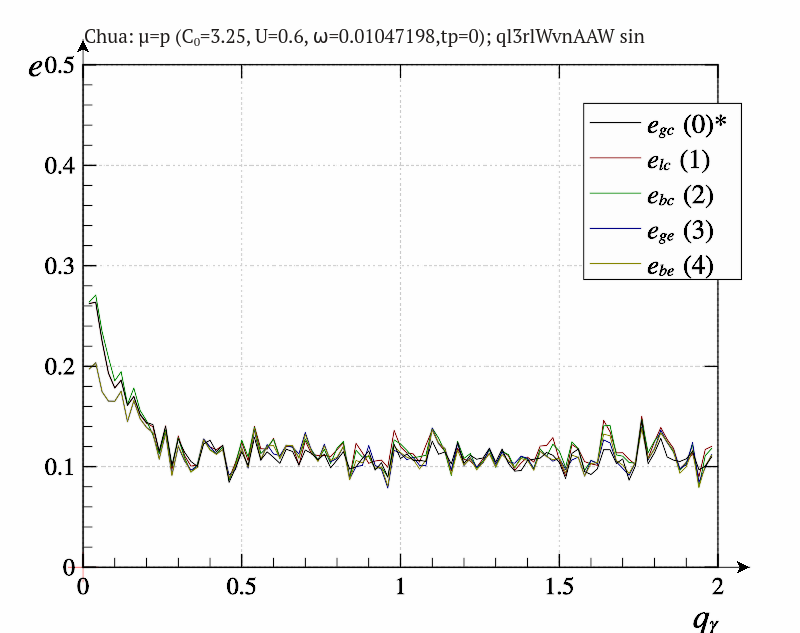
\includegraphics[width=0.49\textwidth]{p/cha/chua/ql3rlWvnAAW/chua_id-p_q_gamma_sin.png}
  }
\caption{Залежності $ \overline{e} (q_\gamma) $ для системи (\ref{atu:eq:chua2}) при умовах (\ref{atu:eq:chua_mu_sign}) і (\ref{atu:eq:chua_mu_sin})
}
\label{atu:f:chua_e_qgamma}
\end{figure}

Явно вираженого екстремуму не спостерігається, що свідчить про
сильну робастність методу. За умов стрибкоподібної динаміки
параметра, похибки, пов'язані з динамікою системи, маскують
цю залежність. За умов (\ref{atu:eq:chua_mu_sin}) виявляється збільшення
рівня помилок при надмірній чутливості функції якості, і та
близьке до рівномірного ``плато'' при її зниженні.

Залежності похибки ідентифікації від коефіцієнта швидкості пошуку
$ v_f $ наведені на рис.~\ref{atu:f:chua_e_v_f}.

\begin{figure}[htb!]
  \centerline{
    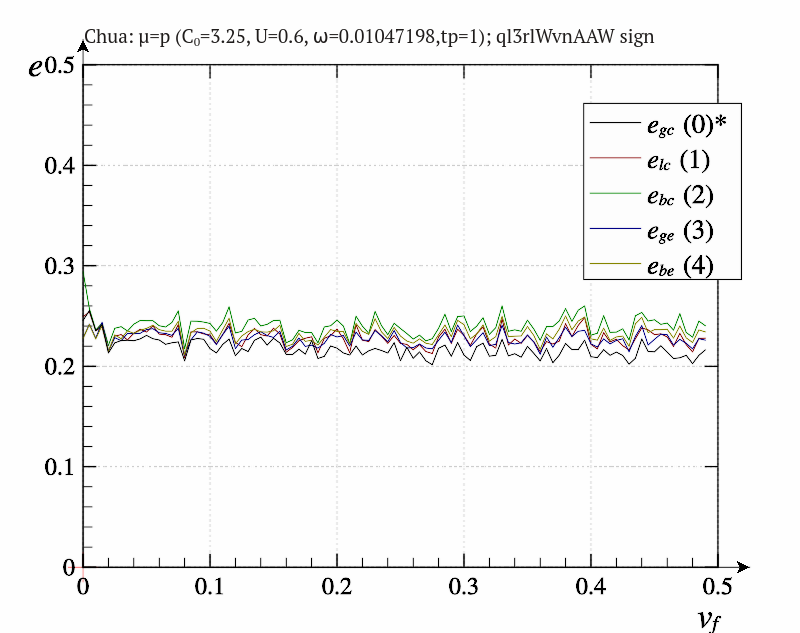
\includegraphics[width=0.49\textwidth]{p/cha/chua/ql3rlWvnAAW/chua_id-p_v_f_sign.png}
    \hfill
    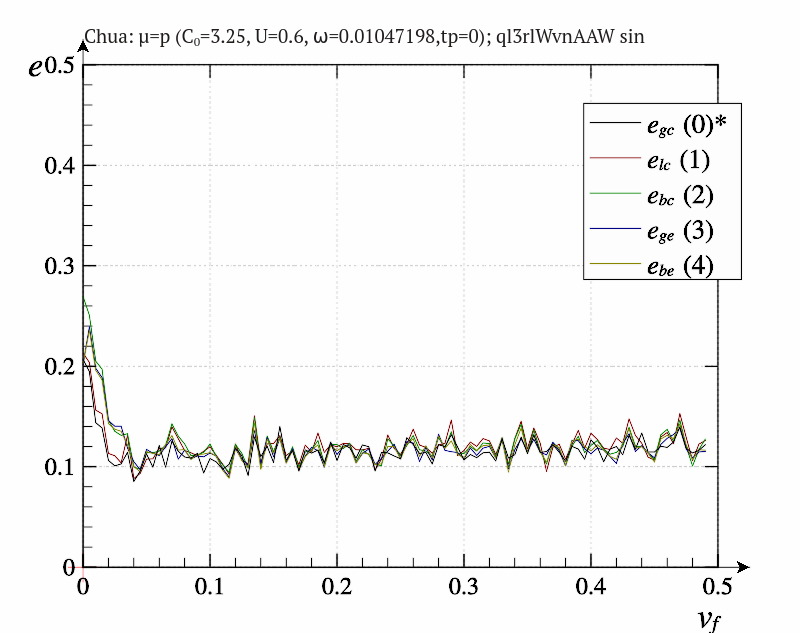
\includegraphics[width=0.49\textwidth]{p/cha/chua/ql3rlWvnAAW/chua_id-p_v_f_sin.png}
  }
\caption{Залежності $ \overline{e} (v_f) $ для системи (\ref{atu:eq:chua2}) при умовах (\ref{atu:eq:chua_mu_sign}) і (\ref{atu:eq:chua_mu_sin})}
\label{atu:f:chua_e_v_f}
\end{figure}

Зниження похибки ідентифікації за рахунок динаміки агентів в
разі плавної зміни параметра
$ \mu $ досягає 250\%. Якщо ж динаміка агентів задана (\ref{atu:eq:chua_mu_sign}),
то виграш істотно нижче.

Залежності
$\overline{e}(k_e)$,
$\overline{e}(k_{nl})$ та
$\overline{e}(k_{cl})$
мають вигляд, абсолютно аналогічний тому, що був отриманий для
інших систем хаотичної динаміки.



% }}}2


\subsection{Висновки} %{{{ 2

Результати моделювання процесів ідентифікації параметра ``$\mu$''
системи Чуа, і порівняння цих результатів з даними, отриманимих
для інших систем, дозволяють зробити наступні висновки:

\begin{itemize}

  \item
    Для ідентифікації параметра
    $ \mu $ системи Чуа можна використовувати кілька критеріїв. При
    цьому критерій
    $ q_{V1} $ дозволяє досягти кращих результатів.

  \item
    Використання методу ql3rlWvnleW для даної системи виправдано.

  \item
    Принципових відмінностей процесу ідентифікації від інших
    систем не виявлено.

\end{itemize}


% }}}2


% }}}1

% vim: fdm=marker foldlevel=1 foldignore="%#" fdc=4 ft=tex
